\documentclass[aspectratio=169, 10pt]{beamer}

%% ─── Theme & Colours ────────────────────────────────────────────────────────
\usetheme{Madrid}
\usecolortheme{seahorse}
\setbeamertemplate{navigation symbols}{}
\setbeamertemplate{footline}[frame number]

%% ─── Packages ────────────────────────────────────────────────────────────────
\usepackage{amsmath, amssymb, amsthm}
\usepackage{mathtools}
\usepackage{bm}
\usepackage{xcolor}
\usepackage{booktabs}
\usepackage{tikz}
\usetikzlibrary{arrows.meta, positioning, fit, shapes.geometric}
\usepackage{hyperref}

%% ─── Custom commands ─────────────────────────────────────────────────────────
\newcommand{\NTK}{\Theta^{(L)}_\infty}
\newcommand{\R}{\mathbb{R}}
\newcommand{\E}{\mathbb{E}}
\newcommand{\pin}{p^{\mathrm{in}}}
\newcommand{\fth}{f_\theta}
\newcommand{\Kmat}{\mathbf{K}}
\newcommand{\kgrad}{\nabla_K C}
\newcommand{\highlight}[1]{\textcolor{blue!70!black}{\textbf{#1}}}
\newcommand{\myalert}[1]{\textcolor{red!70!black}{\textbf{#1}}}

%% ─── Title ───────────────────────────────────────────────────────────────────
\title[NTK, Natural Gradient, SR \& Adam]{%
  Neural Tangent Kernel:\\
  Convergence, Generalisation, and Connections to\\
  Natural Gradient, Stochastic Reconfiguration \& Adaptive Optimisers}

\subtitle{Based on Jacot, Gabriel \& Hongler, NeurIPS 2018}

\author{Summary \& Extensions}
\date{\today}

% ─────────────────────────────────────────────────────────────────────────────
\begin{document}
% ─────────────────────────────────────────────────────────────────────────────

\begin{frame}
  \titlepage
\end{frame}

%% ─── Outline ─────────────────────────────────────────────────────────────────
\begin{frame}{Outline}
  \tableofcontents
\end{frame}

% ═════════════════════════════════════════════════════════════════════════════
\section{Motivation \& Background}
% ═════════════════════════════════════════════════════════════════════════════

\begin{frame}{Why Study Neural Network Training Dynamics?}
  \begin{columns}[T]
    \begin{column}{0.55\textwidth}
      \textbf{Open questions circa 2018:}
      \begin{itemize}
        \item Loss landscape is \highlight{highly non-convex}: many saddle points, potential bad local minima.
        \item Despite over-parametrisation, ANNs \highlight{generalise remarkably well}.
        \item The dynamics of \emph{deep} networks during gradient descent were not understood.
      \end{itemize}
      \vspace{0.4em}
      \textbf{Known connections:}
      \begin{itemize}
        \item At initialisation, infinite-width ANNs $\equiv$ \textbf{Gaussian Processes} (Neal 1996; Lee et al.\ 2018).
        \item Kernel methods achieve comparable performance (Cho \& Saul, 2009).
      \end{itemize}
    \end{column}
    \begin{column}{0.42\textwidth}
      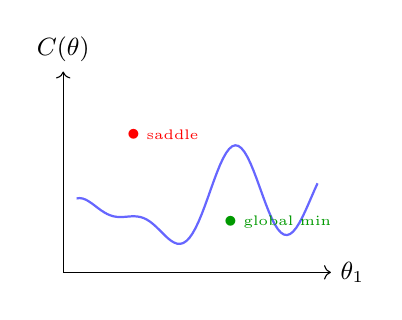
\begin{tikzpicture}[scale=0.85, every node/.style={font=\small}]
        % Schematic loss surface
        \draw[->] (0,0) -- (4,0) node[right]{$\theta_1$};
        \draw[->] (0,0) -- (0,3) node[above]{$C(\theta)$};
        \draw[blue!60, thick, domain=0.2:3.8, samples=80]
          plot (\x, {0.6+0.5*sin(180*\x)+0.3*cos(276.9*\x)+0.2*\x});
        \node[red] at (1.05, 2.05) {$\bullet$};
        \node[red, right] at (1.1, 2.05) {\tiny saddle};
        \node[green!60!black] at (2.5, 0.75) {$\bullet$};
        \node[green!60!black, right] at (2.55, 0.75) {\tiny global min};
      \end{tikzpicture}
      \vspace{0.3em}

      \begin{block}{\small Key Insight}
        Study training in \textbf{function space} $\mathcal{F}$, where the cost is \textbf{convex}, rather than in non-convex parameter space.
      \end{block}
    \end{column}
  \end{columns}
\end{frame}

% ─────────────────────────────────────────────────────────────────────────────
\begin{frame}{ANN Setup and Notation}
  \textbf{Fully-connected ANN}, $L$ layers, widths $n_0, n_1, \ldots, n_L$.

  \medskip
  \textbf{Preactivations and activations} ($\ell = 0,\ldots,L-1$):
  \[
    \alpha^{(0)}(x) = x, \qquad
    \tilde\alpha^{(\ell+1)}(x) = \frac{1}{\sqrt{n_\ell}}\, W^{(\ell)}\alpha^{(\ell)}(x) + \beta b^{(\ell)}, \qquad
    \alpha^{(\ell+1)} = \sigma\!\left(\tilde\alpha^{(\ell+1)}\right).
  \]
  Parameters $W^{(\ell)}_{ij}, b^{(\ell)}_j \sim \mathcal{N}(0,1)$ i.i.d.\ at initialisation.

  \medskip
  \begin{columns}[T]
    \begin{column}{0.5\textwidth}
      \textbf{Network function:} $\fth(x) := \tilde\alpha^{(L)}(x;\theta) \in \R^{n_L}$

      \medskip
      \textbf{Function space} $\mathcal{F} = \{f: \R^{n_0}\to\R^{n_L}\}$ with seminorm
      \[
        \langle f,g\rangle_{\pin} = \E_{x\sim\pin}[f(x)^\top g(x)].
      \]
    \end{column}
    \begin{column}{0.47\textwidth}
      \begin{alertblock}{Key normalisation}
        The factor $1/\sqrt{n_\ell}$ is crucial for a consistent infinite-width limit. It ensures that preactivations remain $\mathcal{O}(1)$ as width grows.
      \end{alertblock}
    \end{column}
  \end{columns}
\end{frame}

% ═════════════════════════════════════════════════════════════════════════════
\section{The Neural Tangent Kernel}
% ═════════════════════════════════════════════════════════════════════════════

\begin{frame}{Kernel Gradient Descent}
  For a multi-dimensional kernel $K: \R^{n_0}\times\R^{n_0}\to\R^{n_L\times n_L}$, define the \textbf{kernel gradient}:
  \[
    \kgrad\big|_{f_0}(x) = \frac{1}{N}\sum_{j=1}^N K(x, x_j)\, d|_{f_0}(x_j),
    \qquad \partial_t f^{\mathrm{in}}C\big|_{f_0} = \langle d|_{f_0}, \cdot\rangle_{\pin}.
  \]

  \textbf{Kernel gradient descent} evolves $f(t)$ via:
  \[
    \partial_t f(t) = -\kgrad\big|_{f(t)}.
  \]

  \begin{theorem}[Cost decay]
    \[
      \partial_t C\big|_{f(t)} = -\|d|_{f(t)}\|^2_K \;\leq\; 0.
    \]
    If $K$ is \highlight{positive definite} w.r.t.\ $\|\cdot\|_{\pin}$ and $C$ is convex and bounded below, then $f(t)$ converges to a \highlight{global minimum}.
  \end{theorem}
\end{frame}

% ─────────────────────────────────────────────────────────────────────────────
\begin{frame}{The Neural Tangent Kernel (NTK)}
  During gradient descent on $C\circ F^{(L)}$, the network function evolves as:
  \[
    \partial_t \fth(t) = -\nabla_{\Theta^{(L)}(\theta)} C\big|_{\fth(t)},
  \]
  where the \textbf{Neural Tangent Kernel} is:
  \[
    \boxed{
      \Theta^{(L)}(\theta) = \sum_{p=1}^P \partial_{\theta_p} F^{(L)}(\theta) \otimes \partial_{\theta_p} F^{(L)}(\theta).
    }
  \]

  \begin{columns}[T]
    \begin{column}{0.48\textwidth}
      \textbf{For finite networks:}
      \begin{itemize}
        \item NTK is \myalert{random} at initialisation.
        \item NTK \myalert{varies} during training.
        \item Analysis is delicate.
      \end{itemize}
    \end{column}
    \begin{column}{0.48\textwidth}
      \textbf{In the infinite-width limit:}
      \begin{itemize}
        \item NTK becomes \highlight{deterministic}.
        \item NTK remains \highlight{constant} during training.
        \item Dynamics fully tractable!
      \end{itemize}
    \end{column}
  \end{columns}
\end{frame}

% ─────────────────────────────────────────────────────────────────────────────
\begin{frame}{Infinite-Width Limit: Gaussian Processes}
  \begin{block}{Proposition 1 (Infinite-width GP limit)}
    As $n_1,\ldots,n_{L-1}\to\infty$, the output functions $\fth_k$ tend (in law) to i.i.d.\ centred Gaussian processes with covariance $\Sigma^{(L)}$, defined recursively:
    \[
      \Sigma^{(1)}(x,x') = \frac{1}{n_0}x^\top x' + \beta^2,
    \]
    \[
      \Sigma^{(L+1)}(x,x') = \E_{f\sim\mathcal{N}(0,\Sigma^{(L)})}\!\left[\sigma(f(x))\,\sigma(f(x'))\right] + \beta^2.
    \]
  \end{block}

  \vspace{0.3em}
  This extends Neal (1996) to deep networks. The kernel $\Sigma^{(L)}$ is the \textbf{NNGP kernel}.

  \vspace{0.5em}
  \begin{exampleblock}{Interpretation}
    At initialisation, an infinitely wide ANN is \emph{equivalent} to Bayesian inference with a GP prior — connecting deep learning to classical kernel methods.
  \end{exampleblock}
\end{frame}

% ─────────────────────────────────────────────────────────────────────────────
\begin{frame}{Theorem 1: NTK Convergence at Initialisation}
  \begin{theorem}[Jacot, Gabriel \& Hongler, 2018]
    As $n_1,\ldots,n_{L-1}\to\infty$, the NTK converges \emph{in probability} to a deterministic limit:
    \[
      \Theta^{(L)}(\theta) \;\xrightarrow{\;P\;}\; \NTK \otimes \mathrm{Id}_{n_L}.
    \]
    The scalar kernel $\NTK$ is defined recursively:
    \[
      \Theta^{(1)}_\infty(x,x') = \Sigma^{(1)}(x,x'),
    \]
    \[
      \Theta^{(L+1)}_\infty(x,x') = \Theta^{(L)}_\infty(x,x')\,\dot\Sigma^{(L+1)}(x,x') + \Sigma^{(L+1)}(x,x'),
    \]
    where $\;\dot\Sigma^{(L+1)}(x,x') = \E_{f\sim\mathcal{N}(0,\Sigma^{(L)})}\!\left[\dot\sigma(f(x))\,\dot\sigma(f(x'))\right]$.
  \end{theorem}

  \vspace{0.3em}
  \textbf{The limiting NTK depends only on:} depth $L$, nonlinearity $\sigma$, initialisation variance.
\end{frame}

% ─────────────────────────────────────────────────────────────────────────────
\begin{frame}{Theorem 2: NTK Stays Constant During Training}
  \begin{theorem}[Stability of NTK under training]
    Under mild regularity assumptions on $\sigma$, and for any $T$ such that $\int_0^T \|d_t\|_{\pin}\,dt$ stays stochastically bounded, as $n_1,\ldots,n_{L-1}\to\infty$:
    \[
      \Theta^{(L)}(t) \;\xrightarrow{\;P\;}\; \NTK \otimes \mathrm{Id}_{n_L}, \quad \text{uniformly for } t\in[0,T].
    \]
  \end{theorem}

  \vspace{0.3em}
  \textbf{Consequence:} In the infinite-width limit, ANN gradient descent \emph{is} kernel gradient descent with a \highlight{fixed kernel} $\NTK$:
  \[
    \partial_t \fth(t) = \Phi_{\NTK\otimes\mathrm{Id}}\!\left(\langle d_t, \cdot\rangle_{\pin}\right).
  \]

  \begin{columns}[T]
    \begin{column}{0.5\textwidth}
      \begin{alertblock}{Mechanistic picture}
        Individual neuron activations change little, but their \emph{collective} variation drives learning in lower layers.
      \end{alertblock}
    \end{column}
    \begin{column}{0.47\textwidth}
      \small
      In the NTK recursion $\Theta^{(L+1)}_\infty = \Theta^{(L)}_\infty\dot\Sigma^{(L+1)} + \Sigma^{(L+1)}$:\\[2pt]
      $\Sigma^{(L+1)}$ $\to$ learning in last layer,\\
      $\Theta^{(L)}_\infty\dot\Sigma^{(L+1)}$ $\to$ learning in lower layers.
    \end{column}
  \end{columns}
\end{frame}

% ═════════════════════════════════════════════════════════════════════════════
\section{Convergence \& Generalisation}
% ═════════════════════════════════════════════════════════════════════════════

\begin{frame}{Least-Squares Regression: Exact Solution}
  For the cost $C(f) = \tfrac12\|f - f^*\|^2_{\pin}$, the dynamics reduce to a \textbf{linear ODE}:
  \[
    \partial_t f_t = \Phi_K\!\left(\langle f^* - f_t, \cdot\rangle_{\pin}\right) = -\Pi(f_t - f^*),
  \]
  where $\Pi(f)_k(x) = \frac{1}{N}\sum_{i=1}^N\sum_{k'}f_{k'}(x_i)\,K_{kk'}(x_i, x)$.

  \vspace{0.3em}
  \textbf{Exact solution:}
  \[
    \boxed{f_t = f^* + e^{-t\Pi}(f_0 - f^*)}.
  \]

  Decomposing along eigenfunctions $f^{(i)}$ of $\Pi$ with eigenvalues $\lambda_i$:
  \[
    f_t = f^* + \Delta^0_f + \sum_{i=1}^{Nn_L} e^{-\lambda_i t}\,\Delta^i_f.
  \]

  \begin{exampleblock}{Key observation}
    Convergence is \emph{fastest} along directions with \highlight{largest eigenvalues} $\lambda_i$ — the leading kernel principal components of the data.
  \end{exampleblock}
\end{frame}

% ─────────────────────────────────────────────────────────────────────────────
\begin{frame}{Generalisation and Early Stopping}
  \begin{columns}[T]
    \begin{column}{0.52\textwidth}
      As $t\to\infty$, the solution converges to:
      \[
        f_{\infty,k}(x) = \kappa^\top_{x,k}\,\tilde K^{-1} y^* + \underbrace{\left(f_{0}(x) - \kappa^\top_{x,k}\tilde K^{-1}y_0\right)}_{\text{centred Gaussian, zero on data}},
      \]
      where $\tilde K = (K_{kk'}(x_i,x_j))$ is the Gram matrix.

      \vspace{0.4em}
      The \textbf{mean} $\kappa^\top_{x,k}\tilde K^{-1}y^*$ equals:
      \begin{itemize}
        \item \textbf{MAP estimate} with GP prior $f_k\sim\mathcal{N}(0,\NTK)$.
        \item \textbf{Kernel ridge regression} (regularisation $\lambda\to 0$).
      \end{itemize}
    \end{column}
    \begin{column}{0.45\textwidth}
      \begin{block}{Motivation for Early Stopping}
        \begin{itemize}
          \item Low-$\lambda_i$ directions correspond to \myalert{high-frequency / noisy} components (e.g.\ high-frequency modes for RBF kernel).
          \item Early stopping halts training before fitting these directions.
          \item $\Rightarrow$ implicit regularisation towards \highlight{smooth, low-complexity} solutions.
        \end{itemize}
      \end{block}
    \end{column}
  \end{columns}
\end{frame}

% ─────────────────────────────────────────────────────────────────────────────
\begin{frame}{Numerical Evidence}
  \begin{columns}[T]
    \begin{column}{0.48\textwidth}
      \textbf{NTK convergence (unit circle, $L=4$):}
      \begin{itemize}
        \item Wider networks: smaller NTK variance, smoother kernel.
        \item Training causes NTK to ``inflate'' for finite-width; negligible for $n=10\,000$.
      \end{itemize}
      \vspace{0.4em}
      \textbf{Kernel regression distribution:}
      \begin{itemize}
        \item Network output distribution at convergence closely matches theoretical GP, even for $n=50$.
      \end{itemize}
    \end{column}
    \begin{column}{0.48\textwidth}
      \textbf{Principal component convergence (MNIST):}
      \begin{itemize}
        \item Eigenvalues: $\lambda_1 \gg \lambda_2 \approx \lambda_3$.
        \item Wider networks converge more \emph{linearly} (in function space) toward $f^*$.
        \item \myalert{Surprising:} narrower networks appear to converge faster in step count — explained by NTK inflation effectively increasing the learning rate.
      \end{itemize}
    \end{column}
  \end{columns}
\end{frame}

% ═════════════════════════════════════════════════════════════════════════════
\section{Connection to Natural Gradient}
% ═════════════════════════════════════════════════════════════════════════════

\begin{frame}{Natural Gradient — Review}
  \textbf{Ordinary gradient descent} in parameter space:
  \[
    \dot\theta = -\nabla_\theta C(\theta).
  \]
  This is metric-dependent: changing parametrisation changes the path.

  \vspace{0.4em}
  \textbf{Natural gradient} (Amari, 1998) uses the \textbf{Fisher information metric} $F(\theta)$:
  \[
    \boxed{\dot\theta = -F(\theta)^{-1}\nabla_\theta C(\theta)},
    \qquad
    F_{pq}(\theta) = \E_x\!\left[\sum_k \partial_{\theta_p}\log p_\theta(k|x)\,\partial_{\theta_q}\log p_\theta(k|x)\right].
  \]

  \begin{columns}[T]
    \begin{column}{0.5\textwidth}
      \textbf{Key properties:}
      \begin{itemize}
        \item Parametrisation-invariant — acts in the \emph{distribution space}.
        \item Equivalent to steepest descent in the KL-divergence geometry.
        \item Encodes the curvature of the model manifold.
      \end{itemize}
    \end{column}
    \begin{column}{0.47\textwidth}
      \begin{alertblock}{Cost}
        $F(\theta)^{-1}$ is $P\times P$ — prohibitive for large networks. Approximations (K-FAC, EKFAC, \ldots) are needed in practice.
      \end{alertblock}
    \end{column}
  \end{columns}
\end{frame}

% ─────────────────────────────────────────────────────────────────────────────
\begin{frame}{NTK as a Fisher-like Metric}
  The NTK can be written as:
  \[
    \Theta^{(L)}(\theta;x,x') = \sum_p \partial_{\theta_p}F^{(L)}(\theta)(x) \otimes \partial_{\theta_p}F^{(L)}(\theta)(x').
  \]

  Compare with the Fisher matrix evaluated on data:
  \[
    F_{pq}(\theta) = \frac{1}{N}\sum_{i,k} \partial_{\theta_p}f_{\theta,k}(x_i)\,\partial_{\theta_q}f_{\theta,k}(x_i).
  \]

  \vspace{0.3em}
  \begin{columns}[T]
    \begin{column}{0.5\textwidth}
      \textbf{The NTK is the ``push-forward'' of the Fisher metric from parameter space to function space:}
      \[
        \Theta^{(L)}(\theta) = J(\theta)\,J(\theta)^\top,
      \]
      where $J(\theta) = \partial_\theta F^{(L)}(\theta)$ is the Jacobian.
    \end{column}
    \begin{column}{0.47\textwidth}
      \begin{block}{Equivalence statement}
        Natural gradient descent in parameter space $\equiv$ kernel gradient descent in function space w.r.t.\ the NTK:
        \[
          \dot f_\theta = -\NTK\, \partial_f C.
        \]
      \end{block}
    \end{column}
  \end{columns}
\end{frame}

% ─────────────────────────────────────────────────────────────────────────────
\begin{frame}{NTK vs Natural Gradient: Comparison}
  \renewcommand{\arraystretch}{1.4}
  \begin{tabular}{lll}
    \toprule
    & \textbf{Natural Gradient} & \textbf{NTK (infinite width)} \\
    \midrule
    Space & Parameter $\R^P$ & Function $\mathcal{F}$ \\
    Metric & Fisher $F(\theta)$ & $\NTK$ (fixed) \\
    Evolution eq.\ & $\dot\theta = -F^{-1}\nabla_\theta C$ & $\dot f = -\NTK\,\partial_f C$ \\
    Curvature & Changes with $\theta$ & \highlight{Constant} (infinite width) \\
    Convergence & Depends on spectrum of $F$ & Depends on spectrum of $\NTK$ \\
    Practical cost & $\mathcal{O}(P^2)$ inversion & $\mathcal{O}(N^2)$ kernel matrix \\
    \bottomrule
  \end{tabular}

  \vspace{0.5em}
  \textbf{Insight:} In the infinite-width limit, natural gradient descent \emph{automatically} reduces to a fixed-kernel method, removing the need to track curvature changes.
\end{frame}

% ═════════════════════════════════════════════════════════════════════════════
\section{Connection to Stochastic Reconfiguration}
% ═════════════════════════════════════════════════════════════════════════════

\begin{frame}{Stochastic Reconfiguration (SR) — Quantum Context}
  In \textbf{variational Monte Carlo} (VMC), one optimises a parametrised wave function $\Psi_\theta$ to minimise the variational energy $E[\Psi_\theta] = \langle\Psi_\theta|H|\Psi_\theta\rangle / \langle\Psi_\theta|\Psi_\theta\rangle$.

  \vspace{0.4em}
  \textbf{Stochastic Reconfiguration} (Sorella, 1998) updates parameters via:
  \[
    \boxed{\dot\theta = -S(\theta)^{-1}\, g(\theta)},
    \qquad
    S_{pq}(\theta) = \E_{\Psi_\theta}\!\left[O_p^*(x)\, O_q(x)\right] - \E[O_p^*]\E[O_q],
  \]
  where $O_p(x) = \partial_{\theta_p}\log\Psi_\theta(x)$ are the \textbf{logarithmic derivatives}, and $g_p = \partial_{\theta_p}E$.

  \begin{columns}[T]
    \begin{column}{0.5\textwidth}
      \textbf{$S(\theta)$ is the quantum geometric tensor} (overlap matrix / quantum Fisher information):
      \[
        S_{pq} = \mathrm{Re}\left(\langle\partial_p\Psi|\partial_q\Psi\rangle - \langle\partial_p\Psi|\Psi\rangle\langle\Psi|\partial_q\Psi\rangle\right).
      \]
    \end{column}
    \begin{column}{0.47\textwidth}
      \begin{exampleblock}{Geometric interpretation}
        SR is natural gradient descent on the manifold of quantum states, respecting the Fubini-Study metric on the projective Hilbert space.
      \end{exampleblock}
    \end{column}
  \end{columns}
\end{frame}

% ─────────────────────────────────────────────────────────────────────────────
\begin{frame}{SR, Fisher, and the NTK: Unified View}
  All three methods implement \textbf{preconditioned gradient descent} with a metric matrix $M$:

  \vspace{0.3em}
  \renewcommand{\arraystretch}{1.5}
  \begin{tabular}{llll}
    \toprule
    \textbf{Method} & \textbf{Domain} & \textbf{Metric $M$} & \textbf{Update} \\
    \midrule
    Gradient descent & $\R^P$ & $\mathbf{I}$ & $\dot\theta = -\nabla_\theta C$ \\
    Natural gradient & prob.\ models & Fisher $F(\theta)$ & $\dot\theta = -F^{-1}\nabla C$ \\
    Stoch.\ Reconfiguration & quantum states & $S(\theta)$ (QFI) & $\dot\theta = -S^{-1} g$ \\
    \highlight{NTK gradient (inf.\ width)} & function space & $\NTK$ (fixed) & $\dot f = -\NTK\,\partial_f C$ \\
    \bottomrule
  \end{tabular}

  \vspace{0.5em}
  \begin{block}{Unifying observation}
    In all cases the metric encodes the \emph{geometry of the model manifold}. The NTK is special because it \textbf{freezes} in the infinite-width limit, converting a nonlinear optimisation problem into a \emph{linear} one — a property not generally shared by SR or the natural gradient.
  \end{block}
\end{frame}

% ─────────────────────────────────────────────────────────────────────────────
\begin{frame}{SR with Neural Quantum States and NTK}
  Modern VMC uses \textbf{neural quantum states} (NQS, Carleo \& Troyer 2017) — parametrised ANNs for $\Psi_\theta$.

  \vspace{0.3em}
  The SR matrix for an NQS becomes:
  \[
    S_{pq} = \E_{\pi_\theta}\!\left[\partial_{\theta_p}\log|\Psi_\theta|\,\partial_{\theta_q}\log|\Psi_\theta|\right]_c
    \approx \frac{1}{N_s}\sum_{s=1}^{N_s} \bar O_p(x_s)\,\bar O_q(x_s), \quad \bar O_p = O_p - \langle O_p\rangle.
  \]

  \begin{columns}[T]
    \begin{column}{0.5\textwidth}
      \textbf{Connection to NTK:}
      \begin{itemize}
        \item Define $J_{s,p} = \partial_{\theta_p}\log|\Psi_\theta(x_s)|$. Then
          \[S \approx \tfrac{1}{N_s}J^\top J \quad (= \text{empirical NTK!})\]
        \item In the \highlight{infinite-width NQS limit}, $S$ converges to a fixed deterministic kernel $\Theta^{(L)}_\infty$ — the NTK of the network.
        \item SR for wide NQS $\approx$ kernel gradient descent in function space.
      \end{itemize}
    \end{column}
    \begin{column}{0.47\textwidth}
      \begin{alertblock}{Practical implications}
        \begin{itemize}
          \item Spectrum of $S$ (eigenvalue distribution) directly controls SR convergence speed — mirroring the NTK eigenvalue story.
          \item Ill-conditioning of $S$ at near-zero eigenvalues corresponds to \emph{redundant parameters} — diagnosed by the NTK.
          \item Regularisation ($S + \epsilon I$) corresponds to implicit early stopping.
        \end{itemize}
      \end{alertblock}
    \end{column}
  \end{columns}
\end{frame}

% ─────────────────────────────────────────────────────────────────────────────
\begin{frame}{Spectrum and Convergence: SR vs NTK}
  The NTK analysis gives a sharp picture of convergence rates:
  \[
    \|f_t - f^*\|^2 \sim \sum_i e^{-2\lambda_i t}\,|\Delta^i_f|^2.
  \]

  \begin{columns}[T]
    \begin{column}{0.5\textwidth}
      \textbf{For NTK gradient descent:}
      \begin{itemize}
        \item Eigenvalues $\lambda_i$ of $\Pi$ (kernel PCA eigenvalues) set convergence timescales.
        \item Large $\lambda_i$ $\to$ fast convergence in that direction.
        \item Small $\lambda_i$ $\to$ slow convergence (high-frequency modes).
      \end{itemize}

      \vspace{0.3em}
      \textbf{For SR (NQS):}
      \begin{itemize}
        \item Eigenvalues of $S$ set update magnitudes.
        \item Near-zero eigenvalues: over-complete parametrisation.
        \item Shift $S + \epsilon I$ regularises (MINRES-SR, diagonal shift).
      \end{itemize}
    \end{column}
    \begin{column}{0.47\textwidth}
      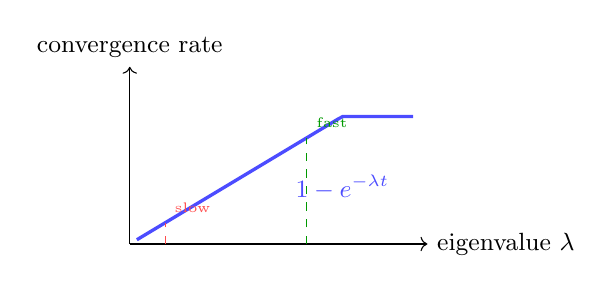
\begin{tikzpicture}[scale=0.9]
        \draw[->] (0,0) -- (4.2,0) node[right]{\small eigenvalue $\lambda$};
        \draw[->] (0,0) -- (0,2.5) node[above]{\small convergence rate};
        \draw[blue!70, very thick, domain=0.1:4, samples=60]
          plot (\x, {min(1.8, 0.6*\x)});
        \draw[dashed, red!70] (0.5, 0) -- (0.5, 0.3) node[above right]{\tiny slow};
        \draw[dashed, green!60!black] (2.5, 0) -- (2.5, 1.5) node[above right]{\tiny fast};
        \node[blue!70] at (3, 0.8) {\small $1-e^{-\lambda t}$};
      \end{tikzpicture}
    \end{column}
  \end{columns}
\end{frame}

% ═════════════════════════════════════════════════════════════════════════════
\section{Neural Tangent Gradients \& Adaptive Optimisers}
% ═════════════════════════════════════════════════════════════════════════════

\begin{frame}{From NTK to Neural Tangent Gradients}
  The NTK describes how the \emph{network function} evolves. But practitioners update
  \emph{parameters} $\theta$ with gradient-based rules. This motivates asking:

  \vspace{0.4em}
  \textbf{What is the parameter-space gradient induced by the NTK?}

  \vspace{0.3em}
  Define the \textbf{Neural Tangent Gradient} (NTG) as the exact gradient of the cost
  projected through the tangent map of the network:
  \[
    \boxed{g^{\mathrm{NT}}_p(t) \;=\; \partial_{\theta_p}C(\theta(t))
      \;=\; \sum_{i,k} \partial_{\theta_p}f_{\theta,k}(x_i)\;\delta_k(x_i)},
  \]
  where $\delta_k(x_i) = \partial_{f_k(x_i)}C$ is the output residual.

  \begin{columns}[T]
    \begin{column}{0.5\textwidth}
      \textbf{Vector form over the dataset:}
      \[
        \mathbf{g}^{\mathrm{NT}} = J(\theta)^\top \bm{\delta},
        \quad J_{(i,k),\,p} = \partial_{\theta_p}f_{\theta,k}(x_i).
      \]
      Here $J\in\R^{Nn_L\times P}$ is the \textbf{full Jacobian} and
      $\bm{\delta}\in\R^{Nn_L}$ stacks the residuals.
    \end{column}
    \begin{column}{0.47\textwidth}
      \begin{block}{Key relationship}
        The NTK is the \emph{Gram matrix} of NTGs:
        \[
          \Theta^{(L)}_{(i,k),(j,k')} = \sum_p g^{\mathrm{NT}}_{p,(i,k)}\,g^{\mathrm{NT}}_{p,(j,k')}.
        \]
        NTK $= J J^\top$ in function space;\; NTG $= J^\top\bm\delta$ in parameter space.
      \end{block}
    \end{column}
  \end{columns}
\end{frame}

% ─────────────────────────────────────────────────────────────────────────────
\begin{frame}{Gradient Descent Through the NTK Lens}
  Ordinary gradient descent in parameter space reads:
  \[
    \theta_{t+1} = \theta_t - \eta\, J(\theta_t)^\top \bm\delta_t.
  \]
  The induced update in \emph{function space} is:
  \[
    f_{\theta_{t+1}}(x) \approx f_{\theta_t}(x) - \eta\,
    \underbrace{J(x,\theta_t)\,J(\theta_t)^\top}_{\Theta^{(L)}(\theta_t;x,\cdot)}\,\bm\delta_t,
  \]
  where $J(x,\theta) = \partial_\theta f_\theta(x)\in\R^{n_L\times P}$.

  \vspace{0.4em}
  \begin{columns}[T]
    \begin{column}{0.52\textwidth}
      \textbf{Implications:}
      \begin{itemize}
        \item The \highlight{effective step size} in function space is \emph{not} $\eta$ but $\eta\,\lambda_{\min}(\Theta)$
              to $\eta\,\lambda_{\max}(\Theta)$, set by the NTK spectrum.
        \item Poor conditioning ($\lambda_{\max}\!\gg\!\lambda_{\min}$) causes
              oscillations in large-eigenvalue directions and stagnation in small ones.
        \item Adaptive optimisers address exactly this mismatch — they
              \highlight{implicitly rescale the NTG} component-wise.
      \end{itemize}
    \end{column}
    \begin{column}{0.45\textwidth}
      \begin{alertblock}{Why a fixed learning rate is suboptimal}
        A single $\eta$ must simultaneously avoid divergence along the
        largest NTK eigenvalue \emph{and} make progress along the smallest.
        The ratio $\kappa = \lambda_{\max}/\lambda_{\min}$ (condition number of $\Theta$)
        controls the difficulty — wide networks with very non-uniform spectra suffer most.
      \end{alertblock}
    \end{column}
  \end{columns}
\end{frame}

% ─────────────────────────────────────────────────────────────────────────────
\begin{frame}{Adam: Gradient-Only Adaptive Learning Rates}
  \textbf{Adam} (Kingma \& Ba, 2015) maintains running estimates of the first and second
  moments of the gradient vector, using only gradient information:

  \vspace{0.3em}
  \begin{columns}[T]
    \begin{column}{0.52\textwidth}
      \textbf{Update rules} (at step $t$, for each parameter $p$):
      \begin{align*}
        m_p^{(t)} &= \beta_1 m_p^{(t-1)} + (1-\beta_1)\,g_p^{(t)}, \\
        v_p^{(t)} &= \beta_2 v_p^{(t-1)} + (1-\beta_2)\,\bigl(g_p^{(t)}\bigr)^2, \\
        \hat m_p   &= \frac{m_p^{(t)}}{1-\beta_1^t}, \quad
        \hat v_p   = \frac{v_p^{(t)}}{1-\beta_2^t}, \\
        \theta_p^{(t+1)} &= \theta_p^{(t)} - \frac{\eta\,\hat m_p}{\sqrt{\hat v_p}+\epsilon}.
      \end{align*}
    \end{column}
    \begin{column}{0.45\textwidth}
      \textbf{What each term does:}
      \begin{itemize}
        \item $m_p$ — exponential moving average of gradients (momentum / bias correction).
        \item $v_p$ — exponential moving average of \emph{squared} gradients (tracks per-parameter curvature).
        \item $1/\sqrt{\hat v_p}$ — \highlight{normalises} the update: large curvature $\Rightarrow$ smaller step.
      \end{itemize}
      \begin{block}{\small Typical values}
        $\beta_1=0.9$,\; $\beta_2=0.999$,\; $\epsilon=10^{-8}$.
      \end{block}
    \end{column}
  \end{columns}
\end{frame}

% ─────────────────────────────────────────────────────────────────────────────
\begin{frame}{Adam as an Implicit NTK Preconditioner}
  \textbf{Key observation:} the diagonal of $J^\top J$ (i.e.\ the per-parameter squared NTG norms)
  governs how much each parameter contributes to the function-space update.

  \vspace{0.3em}
  The \textbf{diagonal Fisher} approximation gives:
  \[
    F_{pp} \approx \E_x\!\left[\bigl(\partial_{\theta_p}f_\theta(x)\bigr)^2\right]
    = \bigl[J^\top J\bigr]_{pp}.
  \]
  Adam's $v_p^{(t)} \approx \E[(g_p^{(t)})^2]$ \textbf{estimates exactly this diagonal}, so:
  \[
    \frac{\eta}{\sqrt{v_p}} \approx \frac{\eta}{\sqrt{F_{pp}}}
    \quad\Leftrightarrow\quad \text{diagonal natural gradient step.}
  \]

  \begin{columns}[T]
    \begin{column}{0.5\textwidth}
      \textbf{In NTK language:}
      \begin{itemize}
        \item Adam rescales the NTG \emph{per-parameter}, adaptively matching the
              local curvature of the NTK without ever forming the full $P\times P$ matrix.
        \item Parameters $\theta_p$ that drive large function-space changes (large $[J^\top J]_{pp}$)
              receive \highlight{smaller effective learning rates}.
        \item Parameters in low-curvature directions receive \highlight{larger steps},
              accelerating progress in small-eigenvalue NTK directions.
      \end{itemize}
    \end{column}
    \begin{column}{0.47\textwidth}
      \begin{exampleblock}{Why Adam works well in practice}
        The NTK spectrum of deep networks is typically very non-uniform.
        Adam's per-coordinate scaling partially corrects for this, acting as a
        cheap diagonal approximation to the full NTK-preconditioned update —
        at cost $\mathcal{O}(P)$ rather than $\mathcal{O}(P^2)$.
      \end{exampleblock}
    \end{column}
  \end{columns}
\end{frame}

% ─────────────────────────────────────────────────────────────────────────────
\begin{frame}{NTG, Adam, and the NTK Spectrum: A Unified View}
  \begin{columns}[T]
    \begin{column}{0.5\textwidth}
      \textbf{Schematic: NTK eigenvalue spectrum}

      \vspace{0.5em}
      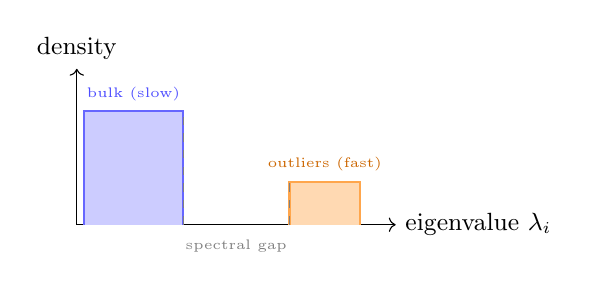
\begin{tikzpicture}[scale=0.9, font=\small]
        \draw[->] (0,0) -- (4.5,0) node[right]{eigenvalue $\lambda_i$};
        \draw[->] (0,0) -- (0,2.2) node[above]{density};
        % bulk
        \fill[blue!20] (0.1,0) rectangle (1.5,1.6);
        \draw[blue!60, thick] (0.1,0) -- (0.1,1.6) -- (1.5,1.6) -- (1.5,0);
        \node[blue!70] at (0.8, 1.85) {\tiny bulk (slow)};
        % outliers
        \fill[orange!30] (3.0,0) rectangle (4.0,0.6);
        \draw[orange!70, thick] (3.0,0) -- (3.0,0.6) -- (4.0,0.6) -- (4.0,0);
        \node[orange!80!black] at (3.5, 0.85) {\tiny outliers (fast)};
        % annotations
        \draw[dashed, gray] (1.5,0) -- (1.5,1.6);
        \draw[dashed, gray] (3.0,0) -- (3.0,0.6);
        \node[gray] at (2.25, -0.3) {\tiny spectral gap};
      \end{tikzpicture}

      \vspace{0.3em}
      \footnotesize
      Bulk: many parameters with small NTG norm $\to$ slow convergence with SGD.\\
      Outliers: few parameters with large NTG norm $\to$ fast convergence but instability risk.
    \end{column}
    \begin{column}{0.47\textwidth}
      \renewcommand{\arraystretch}{1.35}
      \begin{tabular}{p{2.0cm}p{3.5cm}}
        \toprule
        \textbf{Optimiser} & \textbf{Relation to NTK} \\
        \midrule
        SGD & Step $\propto\NTK\,\bm\delta$ (uniform $\eta$, no rescaling) \\
        Momentum & Smooths NTG estimates over time \\
        RMSProp & Diagonal $v_p$ scaling; estimates $[J^\top J]_{pp}$ \\
        \highlight{Adam} & Momentum + diagonal $[J^\top J]_{pp}$ scaling; bias-corrected \\
        Nat.\ Grad.\ / SR & Full $[J^\top J]^{-1}$ in parameter space (exact NTK precond.) \\
        \textbf{NTK GD} & Full $\NTK$ in \emph{function} space (exact, infinite width) \\
        \bottomrule
      \end{tabular}
    \end{column}
  \end{columns}
\end{frame}

% ─────────────────────────────────────────────────────────────────────────────
\begin{frame}{Adam vs NTK: Limitations and Open Questions}
  \begin{columns}[T]
    \begin{column}{0.5\textwidth}
      \textbf{What Adam captures:}
      \begin{itemize}
        \item Diagonal curvature (second moment of NTG).
        \item Temporal smoothing via exponential moving averages.
        \item Bias correction for early-training transients.
        \item Implicit regularisation through bounded effective step sizes.
      \end{itemize}
      \vspace{0.4em}
      \textbf{What Adam misses:}
      \begin{itemize}
        \item \myalert{Off-diagonal NTK structure}: correlations between parameters are ignored.
        \item \myalert{Feature learning}: Adam (like NTK theory) is most natural in the lazy/linear regime; feature learning breaks the fixed-kernel picture.
        \item \myalert{NTK drift}: finite-width networks have a slowly drifting kernel; Adam's $v_p$ tracks this implicitly but inexactly.
      \end{itemize}
    \end{column}
    \begin{column}{0.47\textwidth}
      \begin{block}{Practical guidance from NTK theory}
        \begin{itemize}
          \item \textbf{Learning rate warmup}: the NTK is random at initialisation; warming up $\eta$ lets the kernel stabilise before large steps are taken.
          \item \textbf{Layer-wise learning rates}: different layers have very different NTK eigenvalue scales — separate $\eta$ per layer (or LARS/LAMB) is justified by NTK analysis.
          \item \textbf{Spectral monitoring}: tracking $\|J\|_F$ (Frobenius norm of Jacobian) during training detects NTK drift in finite-width networks.
        \end{itemize}
      \end{block}
    \end{column}
  \end{columns}
\end{frame}

% ─────────────────────────────────────────────────────────────────────────────
\begin{frame}{NTK-Informed Optimisation: Hierarchy of Approximations}
  \begin{center}
  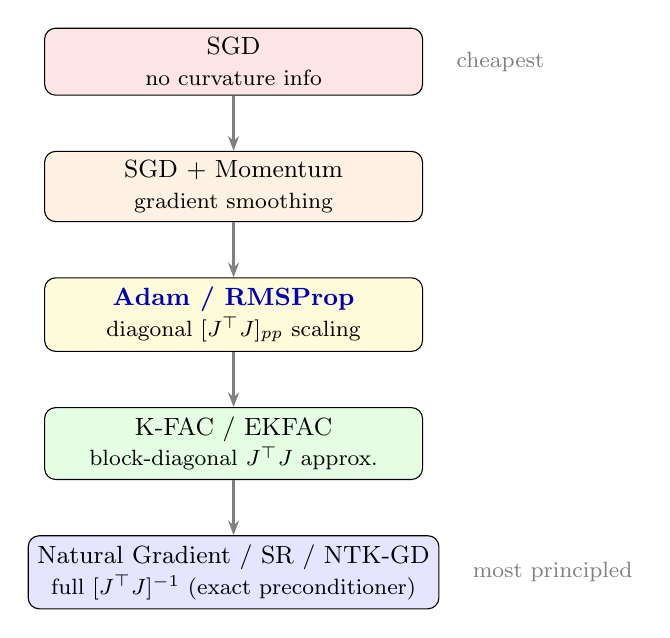
\begin{tikzpicture}[
      node distance=0.7cm and 0.1cm,
      box/.style={draw, rounded corners, align=center, minimum width=4.8cm,
                  minimum height=0.85cm, font=\small},
      col1/.style={box, fill=red!10},
      col2/.style={box, fill=orange!10},
      col3/.style={box, fill=yellow!15},
      col4/.style={box, fill=green!10},
      col5/.style={box, fill=blue!10},
      arr/.style={-{Stealth[scale=0.8]}, thick, gray}
    ]
    \node[col1] (sgd)  {SGD \\ \footnotesize no curvature info};
    \node[col2, below=of sgd] (mom)  {SGD + Momentum \\ \footnotesize gradient smoothing};
    \node[col3, below=of mom] (adam) {\highlight{Adam / RMSProp} \\ \footnotesize diagonal $[J^\top J]_{pp}$ scaling};
    \node[col4, below=of adam] (kfac) {K-FAC / EKFAC \\ \footnotesize block-diagonal $J^\top J$ approx.};
    \node[col5, below=of kfac] (ng)   {Natural Gradient / SR / NTK-GD \\ \footnotesize full $[J^\top J]^{-1}$ (exact preconditioner)};

    \draw[arr] (sgd)  -- (mom);
    \draw[arr] (mom)  -- (adam);
    \draw[arr] (adam) -- (kfac);
    \draw[arr] (kfac) -- (ng);

    \node[right=0.3cm of sgd,  font=\footnotesize, gray] {cheapest};
    \node[right=0.3cm of ng,   font=\footnotesize, gray] {most principled};
  \end{tikzpicture}
  \end{center}

  \vspace{0.2em}
  \small
  Each level approximates the NTK preconditioner more faithfully, at increasing cost.
  \textbf{Adam sits in the sweet spot}: $\mathcal{O}(P)$ memory and compute, strong empirical performance, and a clear theoretical interpretation as a diagonal NTK preconditioner built from gradients alone.
\end{frame}

% ═════════════════════════════════════════════════════════════════════════════
\section{Summary \& Outlook}
% ═════════════════════════════════════════════════════════════════════════════

\begin{frame}{Summary of Main Results}
  \begin{enumerate}
    \setlength\itemsep{0.5em}
    \item \textbf{NTK at initialisation} (Theorem 1): In the infinite-width limit, the NTK converges in probability to a fixed deterministic kernel $\NTK$, depending only on $L$, $\sigma$, and initialisation variance.
    \item \textbf{NTK during training} (Theorem 2): The NTK remains constant throughout training in the infinite-width limit — ANN training becomes \highlight{kernel gradient descent}.
    \item \textbf{Least-squares regression}: The network function satisfies a \textbf{linear ODE}; convergence follows the \highlight{kernel principal components} of the data.
    \item \textbf{Convergence guarantee}: Positive-definiteness of $\NTK$ $\Rightarrow$ convergence to a global minimum.
    \item \textbf{Generalisation}: The limit $f_\infty$ equals kernel ridge regression / MAP estimation under a GP prior.
    \item \textbf{Early stopping}: Justified as avoiding fitting low-eigenvalue (noisy/high-frequency) directions.
  \end{enumerate}
\end{frame}

% ─────────────────────────────────────────────────────────────────────────────
\begin{frame}{Unifying Picture: Geometry of Learning}
  \begin{center}
  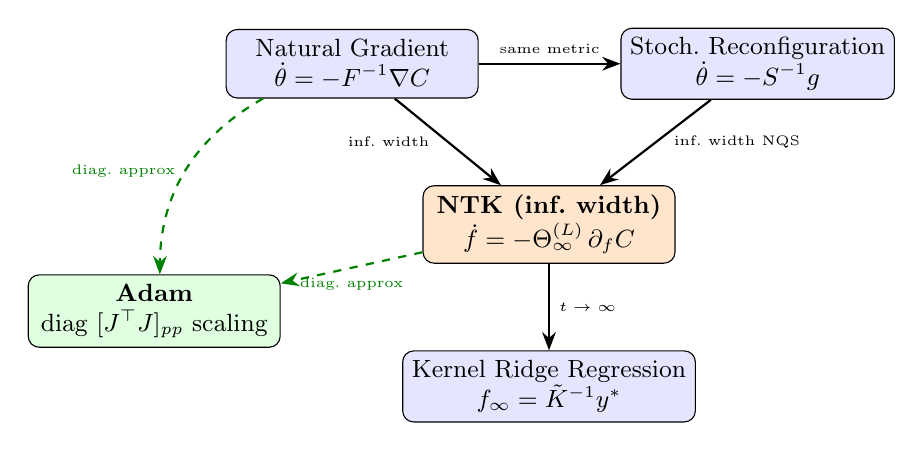
\begin{tikzpicture}[
      node distance=1.1cm and 1.8cm,
      box/.style={draw, rounded corners, fill=blue!10, align=center, minimum width=3.2cm, font=\small},
      hbox/.style={draw, rounded corners, fill=orange!20, align=center, minimum width=3.2cm, font=\small},
      abox/.style={draw, rounded corners, fill=green!12, align=center, minimum width=3.2cm, font=\small},
      arr/.style={-{Stealth}, thick}
    ]
    \node[box] (ng)   {Natural Gradient\\$\dot\theta = -F^{-1}\nabla C$};
    \node[box, right=of ng] (sr)   {Stoch.\ Reconfiguration\\$\dot\theta = -S^{-1}g$};
    \node[hbox, below=of ng, xshift=2.5cm] (ntk)  {\textbf{NTK (inf.\ width)}\\$\dot f = -\NTK\,\partial_f C$};
    \node[abox, left=of ntk, yshift=-1.1cm] (adam) {\textbf{Adam}\\diag $[J^\top J]_{pp}$ scaling};
    \node[box, below=of ntk] (kr)   {Kernel Ridge Regression\\$f_\infty = \tilde K^{-1}y^*$};

    \draw[arr] (ng) -- node[above, font=\tiny]{same metric} (sr);
    \draw[arr] (ng) -- node[left, font=\tiny, xshift=-3pt]{inf.\ width} (ntk);
    \draw[arr] (sr) -- node[right, font=\tiny, xshift=3pt]{inf.\ width NQS} (ntk);
    \draw[arr] (ntk) -- node[right, font=\tiny]{$t\to\infty$} (kr);
    \draw[arr, dashed, green!50!black] (ntk) -- node[below, font=\tiny]{diag.\ approx} (adam);
    \draw[arr, dashed, green!50!black] (ng)  to[bend right=30] node[left, font=\tiny]{diag.\ approx} (adam);
  \end{tikzpicture}
  \end{center}
  \vspace{0.2em}
  All methods share a common foundation: \textbf{preconditioned gradient descent on a Riemannian model manifold}. Adam provides the cheapest gradient-only approximation to the full NTK preconditioner.
\end{frame}

% ─────────────────────────────────────────────────────────────────────────────
\begin{frame}{Open Questions \& Outlook}
  \begin{columns}[T]
    \begin{column}{0.5\textwidth}
      \textbf{Theoretical extensions:}
      \begin{itemize}
        \item Beyond infinite width: \emph{finite-width corrections} (feature learning vs.\ lazy training).
        \item Mean-field / $\mu$P parametrisation (Yang \& Hu, 2021): NTK freezes $\Leftrightarrow$ no feature learning.
        \item NTK for CNNs, attention, transformers.
        \item Sharp sample complexity / generalisation bounds via NTK.
      \end{itemize}
    \end{column}
    \begin{column}{0.47\textwidth}
      \textbf{NQS / SR \& optimiser connections:}
      \begin{itemize}
        \item Infinite-width NQS: does $S$ converge to a fixed kernel?
        \item Can NTK theory guide architecture choices for VMC?
        \item Spectral analysis of $S$ for diagnosis of training pathologies.
        \item Connections to quantum geometry (quantum Fisher, Berry curvature).
        \item NTK-informed adaptive learning rates for SR (diagonal $S$ shift vs.\ full inversion).
      \end{itemize}
    \end{column}
  \end{columns}

  \vspace{0.5em}
  \begin{exampleblock}{Bottom line}
    The NTK provides a \textbf{mathematically rigorous bridge} between deep learning, kernel methods, information geometry, and quantum variational algorithms — a powerful framework for understanding and designing learning systems.
  \end{exampleblock}
\end{frame}

% ─────────────────────────────────────────────────────────────────────────────
\begin{frame}{Key References}
  \footnotesize
  \begin{itemize}
    \item D.P.\ Kingma \& J.\ Ba. \textit{Adam: A Method for Stochastic Optimization.} ICLR 2015.
    \item T.\ Tieleman \& G.\ Hinton. \textit{Lecture 6.5 — RMSProp.} Coursera, 2012.
    \item J.\ Martens \& R.\ Grosse. \textit{Optimizing Neural Networks with Kronecker-factored Approximate Curvature (K-FAC).} ICML 2015.
    \item A.\ Jacot, F.\ Gabriel, C.\ Hongler. \textit{Neural Tangent Kernel: Convergence and Generalization in Neural Networks.} NeurIPS 2018.
    \item R.M.\ Neal. \textit{Bayesian Learning for Neural Networks.} Springer, 1996.
    \item J.H.\ Lee et al.\ \textit{Deep Neural Networks as Gaussian Processes.} ICLR 2018.
    \item S.\ Amari. \textit{Natural Gradient Works Efficiently in Learning.} Neural Computation, 1998.
    \item S.\ Sorella. \textit{Green Function Monte Carlo with Stochastic Reconfiguration.} PRL, 1998.
    \item G.\ Carleo \& M.\ Troyer. \textit{Solving the quantum many-body problem with artificial neural networks.} Science, 2017.
    \item G.\ Yang \& E.J.\ Hu. \textit{Tensor Programs IV: Feature Learning in Infinite-Width Neural Networks.} ICML 2021.
    \item F.\ Becca \& S.\ Sorella. \textit{Quantum Monte Carlo Approaches for Correlated Systems.} Cambridge, 2017.
  \end{itemize}
\end{frame}

% ─────────────────────────────────────────────────────────────────────────────
\begin{frame}[plain]
  \begin{center}
    \Huge Thank you\\[1em]
    \large Questions?
  \end{center}
\end{frame}

\end{document}
